
\subsection{Inverse dynamics - initial velocity}
The objective of this activity is display the UR5 robot on rviz and control the motion of its joints with inverse dynamics control method. The simulation starts with the initial joint position $\begin{bmatrix} \pi & -\frac{\pi}{8} & -\frac{\pi}{6} & 0.0 & 0.0 & 0.0 \end{bmatrix}$ rad and joint velocity $\begin{bmatrix} 0.0 & 0.4\pi & 0.0 & 0.0 & 1.2\pi & 0.0 \end{bmatrix}$. The second and fifth joints will move following a sinusoidal trajectory during the first 4 seconds and maintain a constant joint position during the last second. Finally, the rosnode file that control the movement of the six joints of UR5 robot is the same as Algorithm \ref{lst:inverse_dynamics_control} except that the initial velocity of the robot matches desired initial velocity. Figure  \ref{fig:act_2.2_de} shows the joint velocity error of each joint. In this figure, the velocity of second and fifth joints are equal to $0$ $\mathrm{\frac{rad}{s}}$ expect when the reference trajectory change from sinusoidal to constant value. 
\vspace{20px}

\begin{figure}[H]
    \centering
    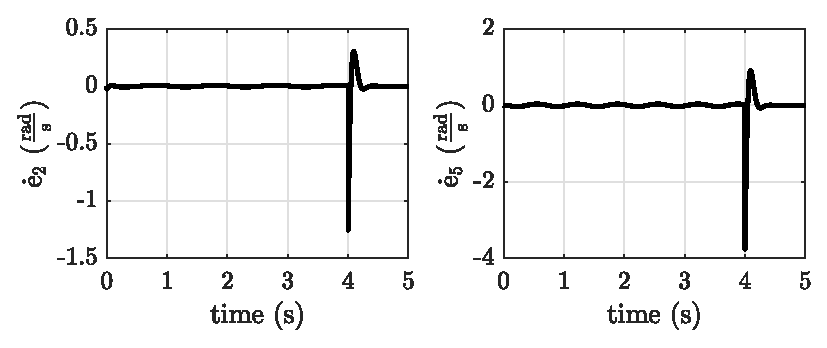
\includegraphics{images/act_2.2/de.eps}
    \caption{Angular velocity error of each joint of UR5 robot with Algorithm \ref{lst:inverse_dynamics_control} and equal initial velocity for robot and reference.}
    \label{fig:act_2.2_de}
\end{figure}